\documentclass[tikz]{standalone}
\usetikzlibrary{graphs}
\begin{document}
\begin{tikzpicture} %简单直线 
	\begin{tikzpicture}
		\draw (0,0) -- (1,1);
	\end{tikzpicture}
\end{tikzpicture}

\begin{tikzpicture}
	\draw (0,0) -- (1,1);
\end{tikzpicture}

%还可以这样写命令,直接在文本中显示直线 
\tikz \draw (0,0) -- (1,1);

%在直线上标注 \\
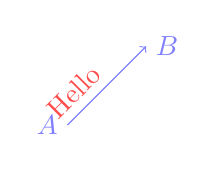
\begin{tikzpicture}
	\draw [color=blue!50, ->](0,0) node[left]{$A$}-- node [color=red!70,pos=0.25,above,sloped]{Hello}(1,1) node[right]{$B$};
\end{tikzpicture}

\begin{tikzpicture}
	\draw [color=blue!50, ->](0,0) node[left]{$A$}-- node [color=red!70,pos=0.25,above,sloped]{Hello}(3,3) node[right]{$B$};
\end{tikzpicture}

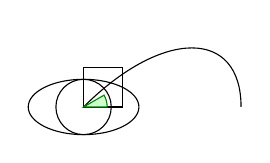
\begin{tikzpicture}
	\draw (0,0) circle (10pt);
	\draw (0,0) .. controls (1,1) and (2,1) .. (2,0);
	\draw (0,0) ellipse (20pt and 10pt);
	\draw (0,0) rectangle (0.5,0.5);
	\filldraw[fill=green!20!white, draw=green!50!black](0,0) -- (3mm,0mm) arc (0:30:3mm) -- cycle;
\end{tikzpicture}

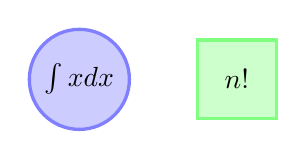
\begin{tikzpicture}
	[L1Node/.style = {circle, draw=blue!50, fill=blue!20, very thick, minimum size=10mm}, L2Node/.style={rectangle, draw=green!50, fill=green!20,very thick, minimum size=10mm}]
		\node[L1Node] (n1) at (0,0){$\int x dx $};
		\node[L2Node] (n2) at (2,0){$n!$};
\end{tikzpicture}

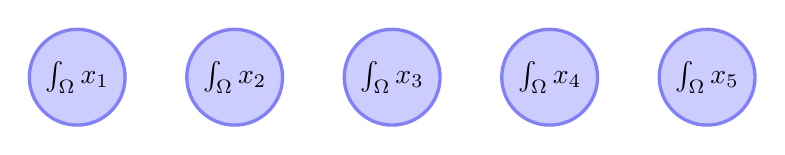
\begin{tikzpicture}
	[L1Node/.style = {circle, draw=blue!50, fill=blue!20, very thick, minimum size=10mm}, L2Node/.style={rectangle, draw=green!50, fill=green!20,very thick, minimum size=10mm}]
 	\foreach \x in {1,...,5}
	\node[L1Node] (w1_\x) at (2*\x, 0){$\int_\Omega x_\x$};
\end{tikzpicture}

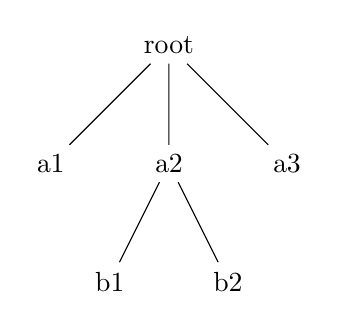
\begin{tikzpicture}
	\node {root}
		child {node {a1}}
		child {node {a2}
			child {node {b1}}
			child {node {b2}}}
		child {node {a3}};
\end{tikzpicture}

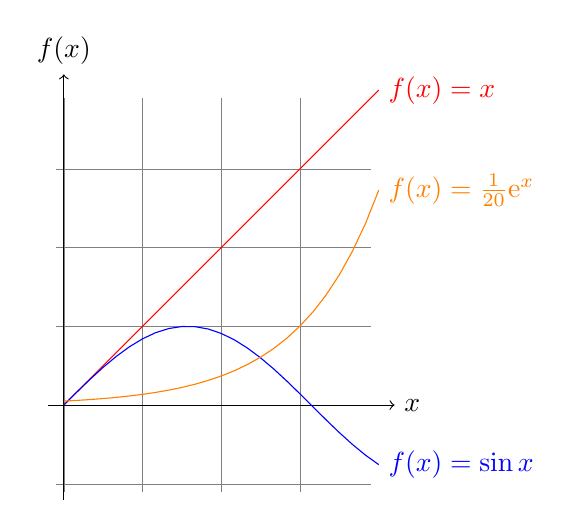
\begin{tikzpicture}[domain=0:4]
	\draw[very thin, color=gray] (-0.1,-1.1) grid (3.9, 3.9);
	\draw[->] (-0.2,0) -- (4.2,0) node[right] {$x$};
	\draw[->] (0,-1.2) -- (0,4.2) node[above] {$f(x)$};
	\draw[color=red] plot(\x,\x) node[right] {$f(x)=x$};
	% \x r 表示弧度
	\draw[color=blue] plot(\x,{sin(\x r)}) node[right] {$f(x) =\sin x$};
	\draw[color=orange] plot(\x, {0.05*exp(\x)}) node[right] {$f(x) = \frac{1}{20} \mathrm e^x$};
\end{tikzpicture}

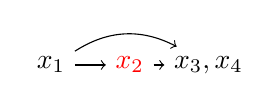
\begin{tikzpicture}
	\graph {
		"$x_1$"-> "$x_2$"[red]-> "$x_3,x_4$";
		"$x_1$"-> [bend left] "$x_3,x_4$";
		};
\end{tikzpicture}

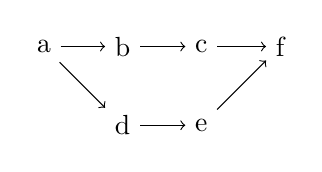
\begin{tikzpicture}
	\graph {
		a-> {
			b->c,
			d->e
		}->f
		};
\end{tikzpicture}

\end{document}
